\documentclass[aspectratio=169,10pt]{beamer}

\usetheme{metropolis}
\usepackage{appendixnumberbeamer}
\usepackage{booktabs}
\usepackage{amsmath,amssymb}
\usepackage{tikz}
\usetikzlibrary{arrows.meta,positioning,calc,decorations.pathreplacing,shapes.geometric,fit}
\usepackage{pgfplots}
\pgfplotsset{compat=1.18}
\usepackage{xcolor}
\usepackage{multicol}
\usepackage{graphicx}
\usepackage{hyperref}
\hypersetup{colorlinks=true,urlcolor=columbia,linkcolor=columbia}

% Columbia-inspired palette (matching L21)
\definecolor{columbia}{RGB}{29,79,145}
\definecolor{columbialight}{RGB}{117,170,219}
\definecolor{columbiaaccent}{RGB}{210,73,42}
\definecolor{columbiagray}{RGB}{117,117,117}
\definecolor{softbg}{RGB}{245,245,250}
\definecolor{hlgreen}{RGB}{46,139,87}

\setbeamercolor{frametitle}{bg=columbia,fg=white}
\setbeamercolor{progress bar}{fg=columbiaaccent}
\setbeamercolor{alerted text}{fg=columbiaaccent}
\setbeamercolor{block title}{bg=columbia,fg=white}
\setbeamercolor{block body}{bg=softbg}

\setbeamerfont{title}{size=\Large,series=\bfseries}
\setbeamerfont{subtitle}{size=\normalsize}

\graphicspath{{./figures/}}

\title{Lecture 22: Clinical Imaging --- Modeling}
\subtitle{BINF 4002 --- Machine Learning for Health}
\author{Matthew McDermott}
\institute{Dept.\ of Biomedical Informatics, Columbia University}
\date{April 9, 2026}

\begin{document}

% ============================================================
\begin{frame}[noframenumbering]
\maketitle
\end{frame}

% ============================================================
\begin{frame}{Where We Are}
\textbf{Modality progression:}
\begin{itemize}
    \item[\textcolor{columbiagray}{$\bullet$}] L17--18: EHR \& Claims \quad\textcolor{columbiagray}{$\bullet$} L19--20: Clinical Text \& NLP
    \item[\textcolor{columbiagray}{$\bullet$}] L21 (Tue): Clinical Imaging --- \textbf{Data}
    \item[\textcolor{columbiaaccent}{$\to$}] \alert{L22: Clinical Imaging --- Modeling} $\gets$ \textbf{today}
    \item[\textcolor{columbiagray}{$\circ$}] L23+: Population Health, Omics, Multimodal
\end{itemize}

\vspace{0.2em}
\textbf{Tuesday:} what medical images \emph{are}---physics, economics, metadata, labels.\\
\textbf{Today:} how to \emph{model} them---and where standard ML approaches break.

\vspace{0.2em}
\textbf{Reorganized around what's \emph{unique} here:}

{\small You know CNNs, encoders, attention. We won't re-teach those. Instead: why does label quality dominate? Why does segmentation need a new architecture? Why does pathology need a new problem formulation? Why do standard augmentations break?}
\end{frame}

% ============================================================
\begin{frame}{Recall: The Five-Question Framework (L21)}
Tuesday's framework---today we address the \textbf{modeling consequences}:
\begin{enumerate}
    \item \textbf{Physics} $\to$ determines whether transfer learning from natural images makes sense
    \item \textbf{Acquisition} $\to$ determines dataset size, which drives pre-training strategy
    \item \textbf{Metadata} $\to$ scanner variation causes distribution shift across sites
    \item \textbf{Labels} $\to$ NLP-extracted silver-standard labels set a noise ceiling
    \item \textbf{Pitfalls} $\to$ shortcuts, augmentation validity, evaluation design
\end{enumerate}

\vspace{0.2em}
\textbf{Today's theme:} In most medical imaging settings, data quality, labeling, and evaluation are the \emph{first} bottlenecks. Architecture still matters---but usually after those are under control.
\end{frame}



% ============================================================
\section{Transfer Learning}
% ============================================================

\begin{frame}{Transfer Learning: The Standard Recipe}
\begin{center}
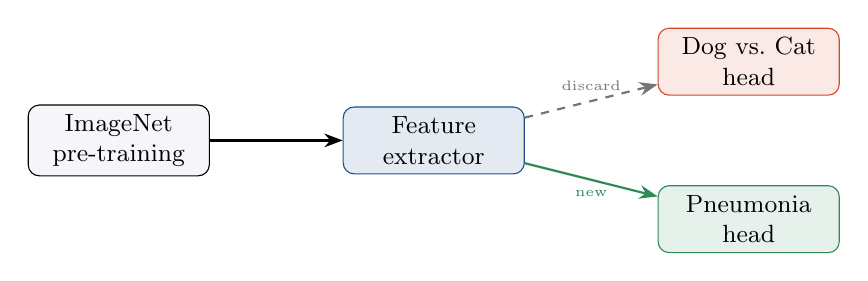
\begin{tikzpicture}[
    box/.style={draw,rounded corners,minimum width=2.3cm,minimum height=0.85cm,align=center,font=\small},
    >=Stealth
]
\node[box,fill=softbg] (inet) at (0,2) {ImageNet\\pre-training};
\node[box,fill=columbia!12,draw=columbia] (feat) at (4,2) {Feature\\extractor};
\node[box,fill=columbiaaccent!12,draw=columbiaaccent] (head1) at (8,3) {Dog vs.\ Cat\\head};
\node[box,fill=hlgreen!12,draw=hlgreen] (head2) at (8,1) {Pneumonia\\head};

\draw[->,thick] (inet) -- (feat);
\draw[->,thick,columbiagray,dashed] (feat) -- (head1) node[midway,above,font=\tiny] {discard};
\draw[->,thick,hlgreen] (feat) -- (head2) node[midway,below,font=\tiny] {new};
\end{tikzpicture}
\end{center}

\vspace{0.2em}
Standard assumption: low-level features transfer across domains. \textbf{But does this actually help?}

{\small Notebook Fig.~1 compares DenseNet features on a natural image vs.\ a chest X-ray.}
\end{frame}

% ============================================================
\begin{frame}{ImageNet Features: Natural vs.\ Medical (Notebook Fig.~1)}
\centering
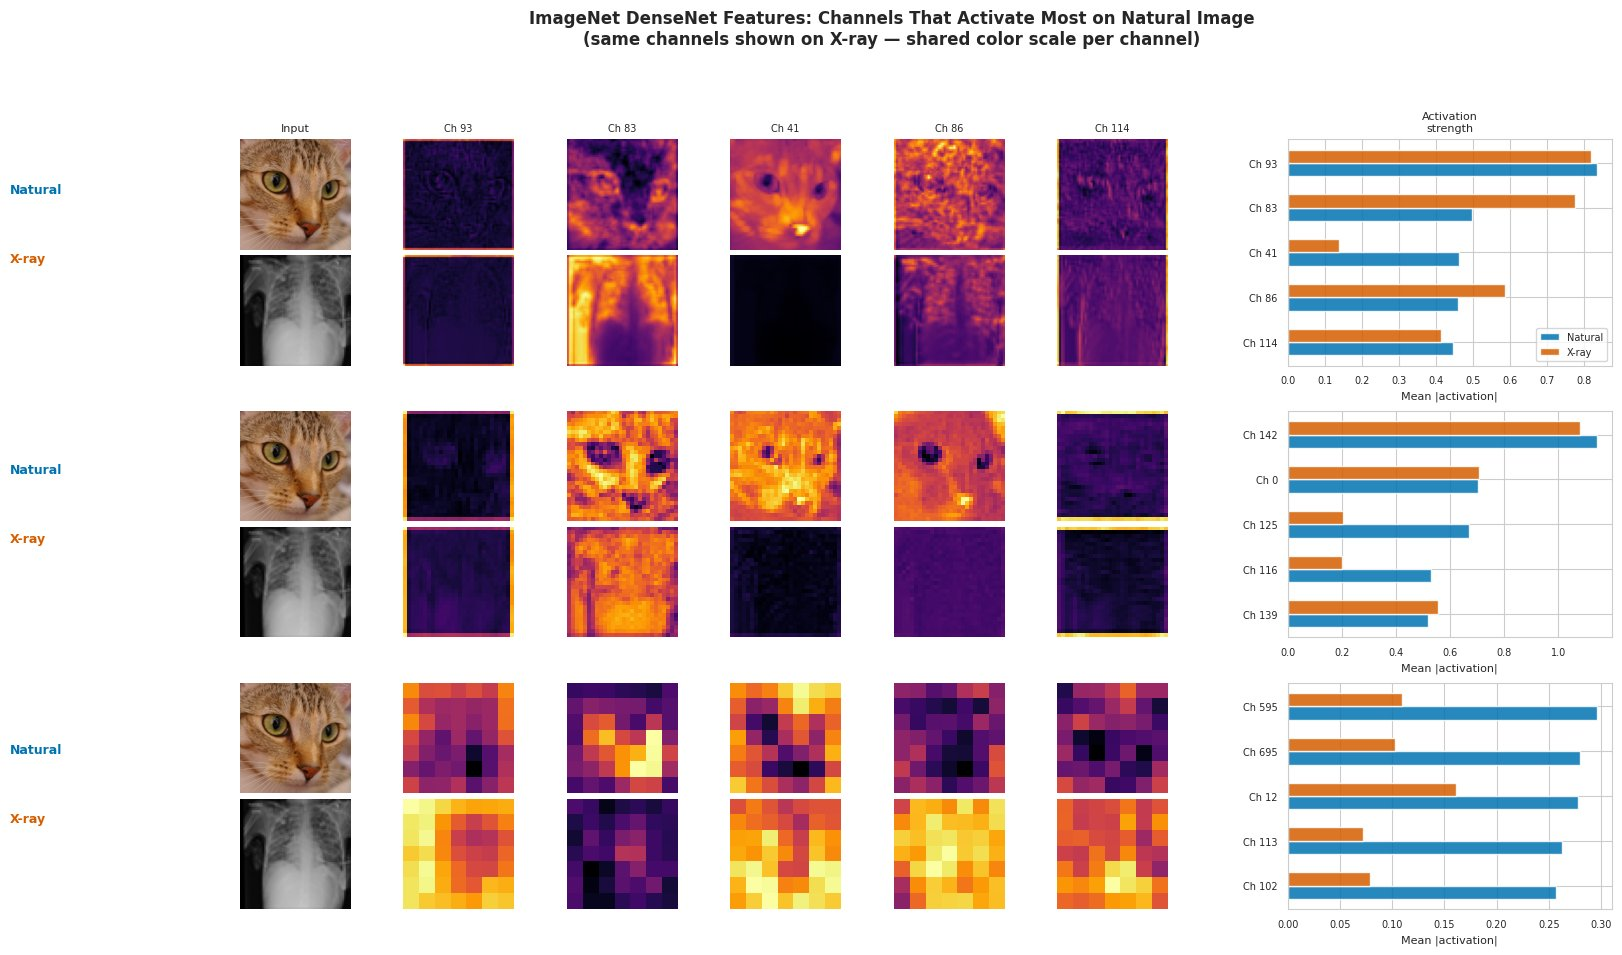
\includegraphics[width=\textwidth,height=0.68\textheight,keepaspectratio]{fig1_feature_comparison.png}

\vspace{-0.3em}
{\scriptsize We pick channels that activate \emph{most strongly on the cat} and show those same channels on the X-ray. \textbf{Early:} both images activate similarly (edges are universal). \textbf{Late:} the cat's top channels are weak on the X-ray---the network doesn't find what it was trained to detect.}

\vspace{0.2em}
{\scriptsize \textbf{Explore:} \url{https://distill.pub/2017/feature-visualization/} \quad \url{https://distill.pub/2018/building-blocks/}}
\end{frame}

% ============================================================
\begin{frame}{Does ImageNet Transfer Actually Help?}
\begin{columns}[T]
\column{0.52\textwidth}
\textbf{Raghu et al., 2019 (``Transfusion''):}
\begin{itemize}[<+->]
    \item Evaluated on retinal disease \& chest X-ray
    \item \alert{Surprising:} little benefit to \textbf{final performance}
    \item Lightweight models matched large ImageNet architectures
    \item Main benefit: \textbf{faster convergence}
    \item Higher layers barely differ from random init
\end{itemize}

\column{0.45\textwidth}
\textbf{Why? Recall L21 (physics):}
\begin{itemize}
    \item Natural: global subjects, RGB, occlusion
    \item Medical: \textbf{local texture}, grayscale, standardized
    \item Only lowest layers retain ImageNet features
\end{itemize}

\begin{block}{Takeaway}
Don't assume transfer helps.\\
\emph{Measure it.} Consider smaller models.
\end{block}
\end{columns}

{\small \textbf{Previous slides:} late features activate weakly on X-rays. Notebook Fig.~2: training curves.}
\end{frame}

% ============================================================
\begin{frame}{Transfusion Results on Real X-Rays (Notebook Fig.~2)}
\centering
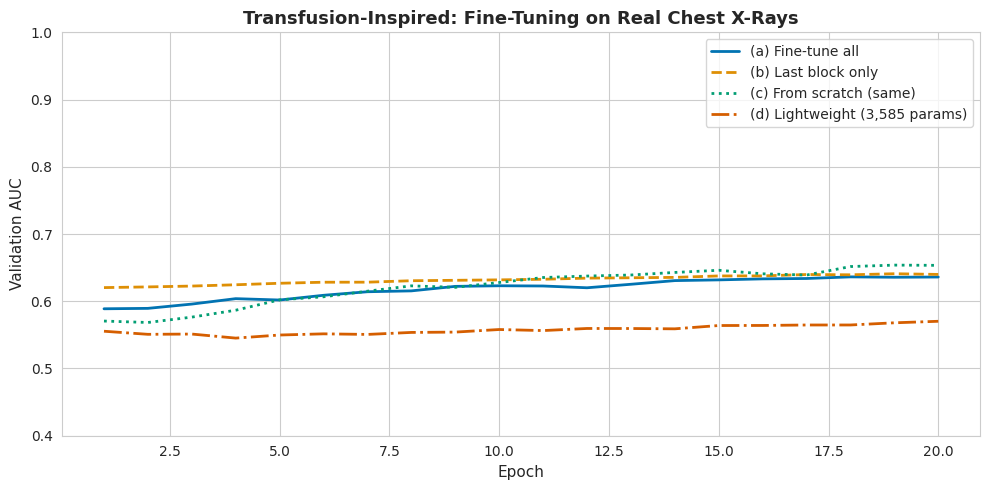
\includegraphics[width=0.85\textwidth]{fig2_finetuning_curves.png}

\vspace{-0.3em}
{\scriptsize Strategies (a)--(c) converge to similar final AUC despite different initialization. The lightweight model (d) is lower---model capacity matters, but pre-training doesn't. This is the Transfusion finding on real ChestMNIST data.}
\end{frame}

% ============================================================
\begin{frame}{When \emph{Does} Pre-training Help?}
\begin{columns}[T]
\column{0.55\textwidth}
\textbf{Domain-specific pre-training:}
\begin{itemize}
    \item Train on large medical corpora \emph{before} fine-tuning
    \item Self-supervised: SimCLR, DINO, MAE---no labels needed
    \item Notable: CheXzero, REMEDIS, CONCH, BiomedCLIP
\end{itemize}

\column{0.42\textwidth}
\begin{block}{Helps Most When\ldots}
\begin{itemize}
    \item Labeled data is small ($<1000$)
    \item Domain features matter (HU, stain)
    \item Task is ``far'' from ImageNet
\end{itemize}
\end{block}

\begin{block}{Matters Less When\ldots}
\begin{itemize}
    \item Large labeled datasets available
    \item Models already over-parametrized
\end{itemize}
\end{block}
\end{columns}

{\small \textbf{Recall L21 (acquisition):} MRI/pathology are expensive $\to$ small data $\to$ pre-training helps. X-ray is cheap $\to$ large data $\to$ less benefit.}
\end{frame}

% ============================================================
\section{The Label Quality Problem}
% ============================================================

\begin{frame}{Label Quality: The Binding Constraint}
This is \textbf{not} a classification-specific problem---it affects every imaging task.

\begin{center}
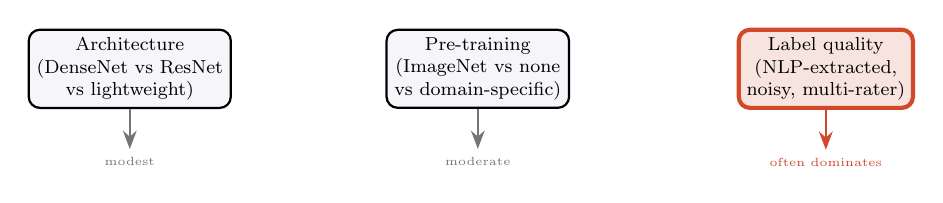
\begin{tikzpicture}[
    box/.style={draw,thick,rounded corners,minimum width=2.4cm,minimum height=0.85cm,align=center,font=\footnotesize},
    >=Stealth,scale=0.85,transform shape
]
\node[box,fill=softbg] (arch) at (0,0) {Architecture\\(DenseNet vs ResNet\\vs lightweight)};
\node[box,fill=softbg] (pretrain) at (5.2,0) {Pre-training\\(ImageNet vs none\\vs domain-specific)};
\node[box,fill=columbiaaccent!15,draw=columbiaaccent,line width=1.5pt] (labels) at (10.4,0) {Label quality\\(NLP-extracted,\\noisy, multi-rater)};

\draw[->,thick,columbiagray] (arch.south) -- ++(0,-0.6) node[below,font=\tiny] {modest};
\draw[->,thick,columbiagray] (pretrain.south) -- ++(0,-0.6) node[below,font=\tiny] {moderate};
\draw[->,thick,columbiaaccent] (labels.south) -- ++(0,-0.6) node[below,font=\tiny,columbiaaccent] {often dominates};
\end{tikzpicture}
\end{center}

\vspace{0.2em}
\textbf{Recall L21 (labels):} Image $\to$ radiologist $\to$ report $\to$ NLP $\to$ label. Each step adds noise. Expert disagreement alone can be substantial. You are training on \emph{labels that are themselves model outputs}.

\vspace{0.2em}
\textbf{Practical implication:} Invest in label quality (adjudication, consensus reads, cleaning NLP labels) rather than architecture search. This applies to classification, segmentation, and MIL equally.
\end{frame}

% ============================================================
\section{Segmentation \& U-Net}
% ============================================================

\begin{frame}{Segmentation: The Clinical Need}
\textbf{Goal:} Assign a class label to every pixel (or voxel).

\vspace{0.2em}
\textbf{Clinical applications:} Tumor delineation for radiation therapy, organ segmentation for surgical planning, lesion measurement for response tracking.

\vspace{0.2em}
\textbf{Key challenge:} A standard encoder compresses spatial information---but segmentation needs to recover the original resolution.

\begin{center}
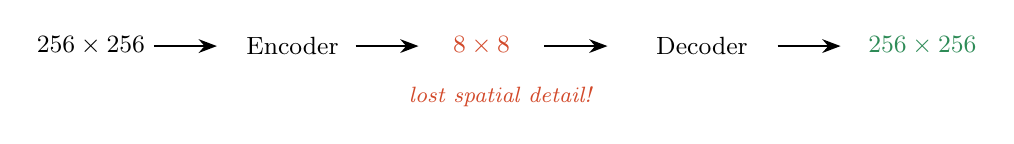
\begin{tikzpicture}[>=Stealth,scale=0.8]
\node[font=\small] at (0,0) {$256\times256$};
\draw[->,thick] (1,0) -- (2,0);
\node[font=\small] at (3.2,0) {Encoder};
\draw[->,thick] (4.2,0) -- (5.2,0);
\node[font=\small,columbiaaccent] at (6.2,0) {$8\times8$};
\draw[->,thick] (7.2,0) -- (8.2,0);
\node[font=\small] at (9.7,0) {Decoder};
\draw[->,thick] (10.9,0) -- (11.9,0);
\node[font=\small,hlgreen] at (13.2,0) {$256\times256$};
\node[below,font=\footnotesize\itshape,columbiaaccent] at (6.5,-0.5) {lost spatial detail!};
\end{tikzpicture}
\end{center}

\textbf{Why not keep full resolution?} A $512\times512$ feature map with 256 channels = 256\,MB per layer. With 10 layers, you can't fit even one image in GPU memory. Downsampling is necessary---the question is how to recover what you lose.
\end{frame}

% ============================================================
\begin{frame}{Real Segmentation Data: Kvasir-SEG}
\centering
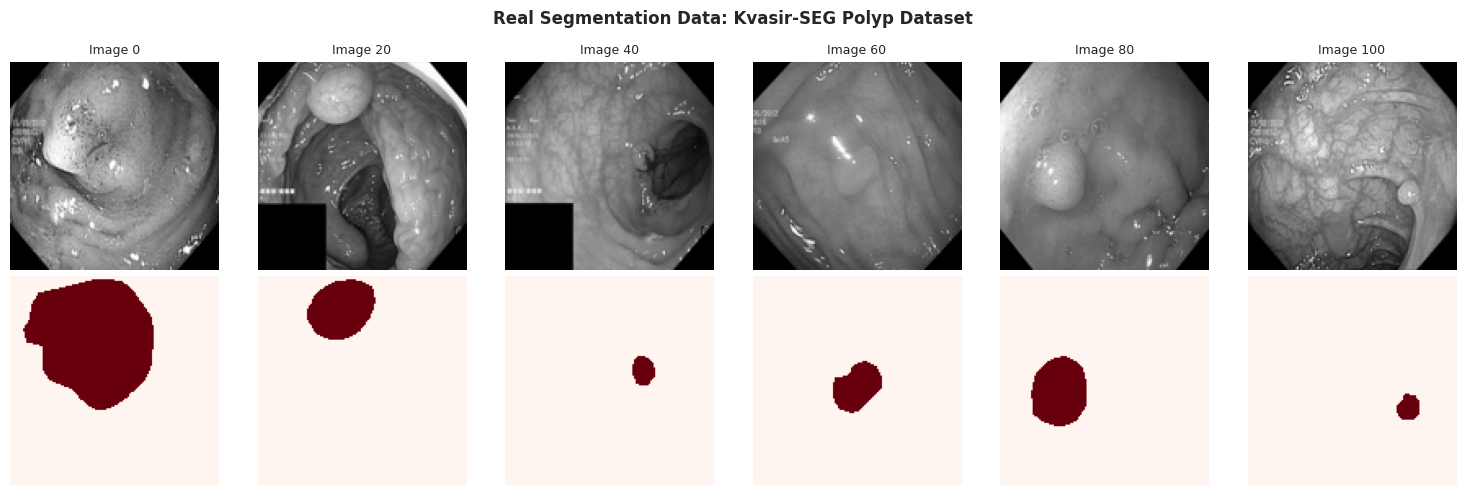
\includegraphics[width=\textwidth,height=0.65\textheight,keepaspectratio]{fig_real_segmentation.png}

\vspace{-0.3em}
{\scriptsize 1{,}000 colonoscopy images with expert polyp masks (Jha et al., 2020). Notice the range of polyp sizes---from large (left) to tiny (right). Small polyps occupy $<$1\% of pixels, making CE loss ineffective. This is the data we train on in the notebook.}
\end{frame}

% ============================================================
\begin{frame}{U-Net: Born in Biomedical Imaging}
\begin{center}
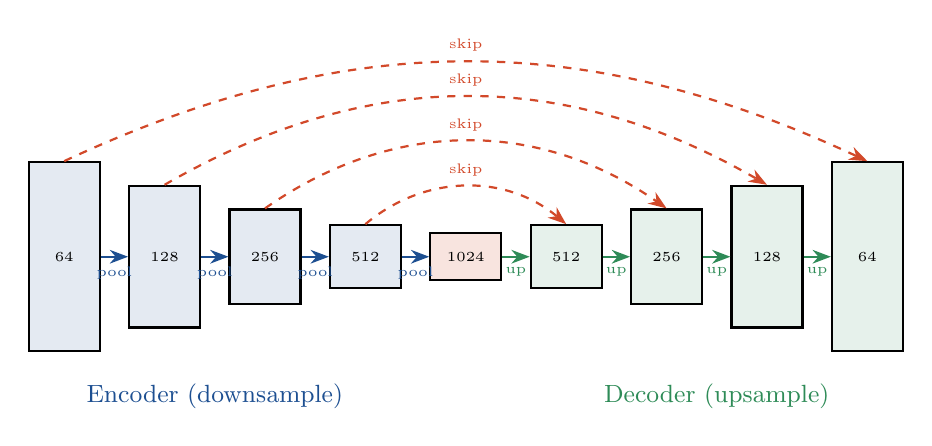
\begin{tikzpicture}[
    encbox/.style={draw,thick,fill=columbia!12,minimum width=0.9cm,font=\tiny,align=center},
    decbox/.style={draw,thick,fill=hlgreen!12,minimum width=0.9cm,font=\tiny,align=center},
    >=Stealth,scale=0.85
]
\node[encbox,minimum height=2.4cm] (e1) at (0,0) {64};
\node[encbox,minimum height=1.8cm] (e2) at (1.5,0) {128};
\node[encbox,minimum height=1.2cm] (e3) at (3,0) {256};
\node[encbox,minimum height=0.8cm] (e4) at (4.5,0) {512};
\node[draw,thick,fill=columbiaaccent!15,minimum width=0.9cm,minimum height=0.6cm,font=\tiny] (bn) at (6,0) {1024};
\node[decbox,minimum height=0.8cm] (d4) at (7.5,0) {512};
\node[decbox,minimum height=1.2cm] (d3) at (9,0) {256};
\node[decbox,minimum height=1.8cm] (d2) at (10.5,0) {128};
\node[decbox,minimum height=2.4cm] (d1) at (12,0) {64};

\draw[->,thick,columbia] (e1) -- (e2) node[midway,below,font=\tiny] {pool};
\draw[->,thick,columbia] (e2) -- (e3) node[midway,below,font=\tiny] {pool};
\draw[->,thick,columbia] (e3) -- (e4) node[midway,below,font=\tiny] {pool};
\draw[->,thick,columbia] (e4) -- (bn) node[midway,below,font=\tiny] {pool};
\draw[->,thick,hlgreen] (bn) -- (d4) node[midway,below,font=\tiny] {up};
\draw[->,thick,hlgreen] (d4) -- (d3) node[midway,below,font=\tiny] {up};
\draw[->,thick,hlgreen] (d3) -- (d2) node[midway,below,font=\tiny] {up};
\draw[->,thick,hlgreen] (d2) -- (d1) node[midway,below,font=\tiny] {up};

\draw[->,thick,columbiaaccent,dashed] (e4.north) to[bend left=40] node[above,font=\tiny,columbiaaccent] {skip} (d4.north);
\draw[->,thick,columbiaaccent,dashed] (e3.north) to[bend left=35] node[above,font=\tiny,columbiaaccent] {skip} (d3.north);
\draw[->,thick,columbiaaccent,dashed] (e2.north) to[bend left=30] node[above,font=\tiny,columbiaaccent] {skip} (d2.north);
\draw[->,thick,columbiaaccent,dashed] (e1.north) to[bend left=25] node[above,font=\tiny,columbiaaccent] {skip} (d1.north);

\node[below=0.3cm,font=\small,columbia] at (2.25,-1.4) {Encoder (downsample)};
\node[below=0.3cm,font=\small,hlgreen] at (9.75,-1.4) {Decoder (upsample)};
\end{tikzpicture}
\end{center}

Skip connections \textbf{concatenate} encoder features with decoder features at each resolution.

{\small \textbf{Ronneberger et al., 2015} --- designed for biomedical segmentation with limited data. Dominant 10+ years later. Notebook Fig.~3: U-Net vs.\ no-skip baseline.}
\end{frame}

% ============================================================
\begin{frame}{Skip Connections: U-Net vs.\ ResNet}
You've seen skip connections before---\textbf{residual connections} in ResNet. How do they differ?

\begin{columns}[T]
\column{0.48\textwidth}
\textbf{ResNet (residual):}
\begin{itemize}
    \item $x_{\text{out}} = F(x) \mathbin{\textcolor{columbia}{+}} x$ \quad (additive)
    \item Same resolution throughout
    \item Purpose: gradient flow in deep networks
    \item Skip carries the \emph{same} features
\end{itemize}

\column{0.48\textwidth}
\textbf{U-Net (skip):}
\begin{itemize}
    \item $x_{\text{out}} = G([\,x_{\text{up}}\; \mathbin{\textcolor{columbiaaccent}{||}} \;x_{\text{enc}}\,])$ \quad (concat)
    \item \emph{Across} resolutions (enc $\to$ dec)
    \item Purpose: recover spatial detail lost by pooling
    \item Skip carries \emph{different} features (high-res)
\end{itemize}
\end{columns}

\textbf{Why this matters clinically:}
\begin{itemize}
    \item Without skip: blurry boundaries, small structures lost
    \item With skip: sharp boundaries---radiation planning requires sub-mm precision
\end{itemize}

{\small \textbf{Variants:} 3D U-Net (volumetric), Attention U-Net, nnU-Net (``AutoML for segmentation'').}
\end{frame}

% ============================================================
\begin{frame}{Skip Connection Comparison (Notebook Fig.~3)}
\centering
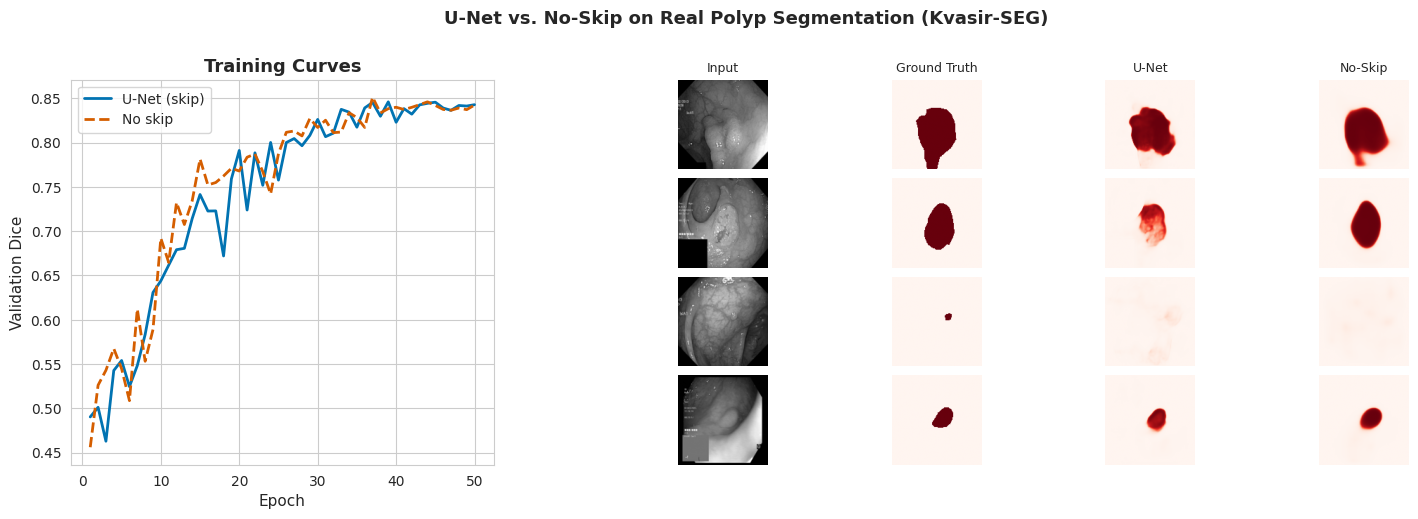
\includegraphics[width=0.85\textwidth]{fig3_unet_comparison.png}

\vspace{-0.3em}
{\scriptsize Real Kvasir-SEG polyps. Dice may be similar---polyps are large. Examine \emph{boundaries}: skip connections preserve edge detail that Dice is insensitive to.}
\end{frame}

% ============================================================
\begin{frame}{Dice Loss: What $\hat{y}$ Means}
\textbf{Problem:} Tumor occupies $<1\%$ of pixels. CE loss: 99\% of the gradient says ``predict background.''

\textbf{Dice loss:} Normalizes by \emph{region size}, not pixel count.
\[
    \mathcal{L}_{\text{Dice}} = 1 - \frac{2\sum_i y_i \hat{y}_i + \epsilon}{\sum_i y_i + \sum_i \hat{y}_i + \epsilon}
\]

\textbf{Important:} $\hat{y}_i = \sigma(z_i) \in [0,1]$ is a \textbf{probability} (sigmoid output), not a hard label. This makes the loss differentiable for training. At evaluation, you threshold ($\hat{y}_i > 0.5$) to get the Dice \emph{coefficient} (= F1 on binary masks).

\textbf{Why Dice focuses on the foreground:} If the foreground has 100 pixels and you miss them all, $\sum y_i \hat{y}_i \approx 0$ so $\mathcal{L}_{\text{Dice}} \approx 1$ regardless of how many of the 9{,}900 background pixels you got right. CE loss would still be $\approx 0.01$---background dominates.

{\small \textbf{In practice:} $\mathcal{L} = \mathcal{L}_{\text{CE}} + \mathcal{L}_{\text{Dice}}$. Notebook Fig.~4: experimental comparison.}
\end{frame}

% ============================================================
\begin{frame}{Loss Function Comparison (Notebook Fig.~4)}
\centering
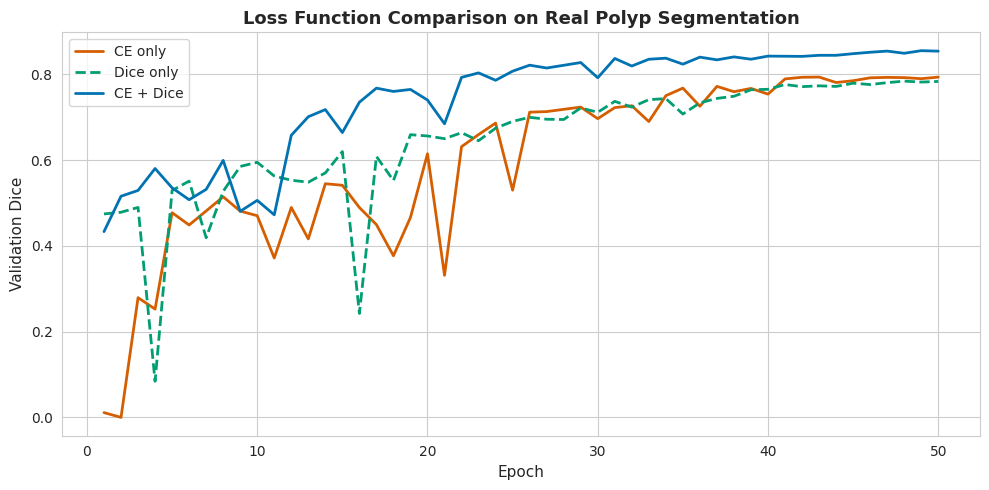
\includegraphics[height=0.60\textheight]{fig4_loss_comparison.png}

\vspace{-0.3em}
{\scriptsize CE+Dice (blue) converges highest and most stably. CE-only (orange) is noisy---gradient dominated by background. Dice-only (green) starts unstable but recovers. Combined loss gets the best of both: stable gradients from CE, foreground focus from Dice.}
\end{frame}

% ============================================================
\section{Whole-Slide Pathology \& MIL}
% ============================================================

\begin{frame}{The Gigapixel Problem}
\textbf{Recall L21 (histopathology):} WSIs are $\sim$100K $\times$ 100K pixels.

\begin{itemize}
    \item Cannot fit in GPU memory (a single slide is $\sim$5\,GB uncompressed)
    \item Labels exist only at the \emph{slide level}: ``this patient has cancer''
    \item You tile the slide into $256\times256$ patches and process each independently
\end{itemize}

\vspace{0.2em}
\begin{center}
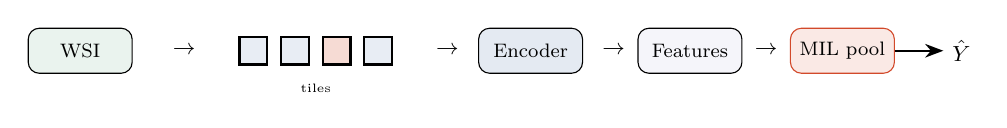
\begin{tikzpicture}[
    box/.style={draw,rounded corners,minimum width=1.5cm,minimum height=0.65cm,align=center,font=\footnotesize},
    tile/.style={draw,thick,minimum width=0.4cm,minimum height=0.4cm},
    >=Stealth,scale=0.88,transform shape
]
\node[box,fill=hlgreen!10] (wsi) at (0,0) {WSI};
\node[font=\small] at (1.5,0) {$\to$};
\foreach \i/\c in {0/columbia!10, 1/columbia!10, 2/columbiaaccent!20, 3/columbia!10} {
    \node[tile,fill=\c] at (2.5+\i*0.6,0) {};
}
\node[below,font=\tiny] at (3.4,-0.35) {tiles};
\node[font=\small] at (5.3,0) {$\to$};
\node[box,fill=columbia!12] at (6.5,0) {Encoder};
\node[font=\small] at (7.7,0) {$\to$};
\node[box,fill=softbg] at (8.8,0) {Features};
\node[font=\small] at (9.9,0) {$\to$};
\node[box,fill=columbiaaccent!12,draw=columbiaaccent] (agg) at (11,0) {MIL pool};
\draw[->,thick] (agg.east) -- ++(0.7,0) node[right,font=\small] {$\hat{Y}$};
\end{tikzpicture}
\end{center}
\end{frame}

% ============================================================
\begin{frame}{MIL: Most Tile Labels Are \emph{Wrong}}
\textbf{The key insight} that makes pathology MIL different from standard classification:

\vspace{0.2em}
A slide labeled ``cancer-positive'' might contain 10{,}000 tiles, of which \emph{maybe 50} actually show cancer. The other 9{,}950 tiles show normal tissue, stroma, fat, or artifacts.

\vspace{0.2em}
If you naively assign the slide label to every tile:
\begin{itemize}[<+->]
    \item 99.5\% of your ``positive'' training labels are \alert{factually wrong}
    \item This isn't label \emph{noise}---it's systematic label \emph{corruption}
    \item Standard classification on these tiles will learn to predict ``cancer'' from normal stroma
\end{itemize}

\vspace{0.2em}
\textbf{MIL formalization:} A bag is positive if \emph{at least one} instance is positive.
\begin{itemize}
    \item Positive bag: $Y_{\text{bag}} = 1 \iff \exists\, i : y_i = 1$ \quad (at least one cancerous tile)
    \item Negative bag: $Y_{\text{bag}} = 0 \iff \forall\, i : y_i = 0$ \quad (all tiles are normal)
\end{itemize}

This is why you need a \emph{pooling} strategy, not per-tile classification.
\end{frame}

% ============================================================
\begin{frame}{MIL Aggregation Strategies}
\textbf{Three strategies:}
\begin{itemize}[<+->]
    \item \textbf{Max-pool:} $h_{\text{bag}} = \max_i h_i$ \quad (most ``positive'' tile wins)
    \item \textbf{Mean-pool:} $h_{\text{bag}} = \frac{1}{N}\sum_i h_i$ \quad (average signal, diluted by 99\% normal tiles)
    \item \textbf{Attention-MIL:} $h_{\text{bag}} = \sum_i \alpha_i h_i$, \; $\alpha_i = \frac{\exp(w^\top h_i)}{\sum_j \exp(w^\top h_j)}$
\end{itemize}

\vspace{0.1em}
\begin{columns}[T]
\column{0.52\textwidth}
\textbf{Attention-MIL (Ilse et al., 2018):}
\begin{enumerate}
    \item Tile features: $h_i = f_\theta(x_i)$
    \item Attention: $a_i = w^\top \tanh(V h_i)$
    \item Normalize: $\alpha_i = \text{softmax}(a_i)$
    \item Aggregate: $h_{\text{bag}} = \sum_i \alpha_i h_i$
    \item Classify: $\hat{Y} = \sigma(W h_{\text{bag}} + b)$
\end{enumerate}

\column{0.45\textwidth}
\textbf{Clinical value of attention:}
\begin{itemize}
    \item Overlay $\alpha_i$ as heatmap on slide
    \item High-attention $\approx$ diagnostic regions
    \item \alert{Caution:} artifacts (pen marks, folds) can dominate attention
\end{itemize}
\end{columns}

{\small Notebook Fig.~5: MIL simulation comparing pooling strategies.}
\end{frame}

% ============================================================
\begin{frame}{MIL Aggregation Comparison (Notebook Fig.~5)}
\begin{center}
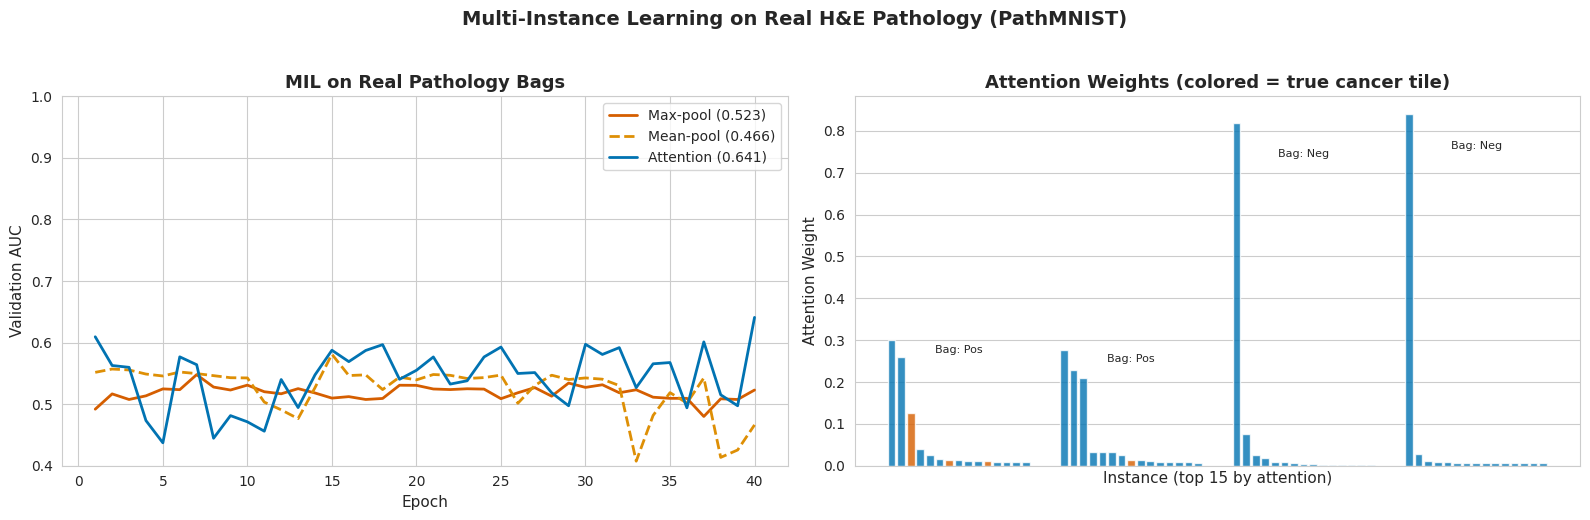
\includegraphics[width=\textwidth,height=0.78\textheight,keepaspectratio]{fig5_mil_comparison.png}
\end{center}
\vspace{-0.3em}
{\scriptsize Left: bag-level AUC on real pathology bags. Attention-MIL learns to focus on the rare diagnostic tiles, outperforming both pooling baselines. Right: attention weights show concentration on specific tiles (tall bars) rather than uniform weighting---the model is learning \emph{where} to look.}
\end{frame}

% ============================================================
\section{Augmentation: Why Physics Matters}
% ============================================================

\begin{frame}{Augmentation: Natural vs.\ Medical Images}
The same augmentation can be valid for natural images and \textbf{invalid for medical images}---because the physics of acquisition differs.

\vspace{0.2em}
\begin{columns}[T]
\column{0.48\textwidth}
\textbf{Vertical flip:}
\begin{itemize}
    \item Natural image of a cat: still a cat $\to$ \textcolor{hlgreen}{\checkmark}
    \item Chest X-ray: heart now on the right $\to$ mimics dextrocardia (a rare clinical finding) $\to$ \textcolor{columbiaaccent}{$\times$}
    \item Pathology tile: no canonical orientation $\to$ \textcolor{hlgreen}{\checkmark}
\end{itemize}

\column{0.48\textwidth}
\onslide<2->{\textbf{Color jitter:}
\begin{itemize}
    \item Natural image: simulates lighting variation $\to$ \textcolor{hlgreen}{\checkmark}
    \item X-ray: grayscale, intensity \emph{is} the signal (tissue density) $\to$ \textcolor{columbiaaccent}{$\times$}
    \item Pathology: simulates stain variation across labs $\to$ \textcolor{hlgreen}{\checkmark}
\end{itemize}}
\end{columns}

\vspace{0.2em}
\textbf{Principle:} An augmentation is valid if and only if it produces images that \emph{could plausibly occur} under the acquisition physics of that modality, without changing the clinical label.

{\small Notebook Fig.~7 applies identical augmentations to a natural image, a chest X-ray, and a pathology tile side-by-side.}
\end{frame}

% ============================================================
\begin{frame}{Augmentation Validity: Real Images (Notebook Fig.~7)}
\begin{center}
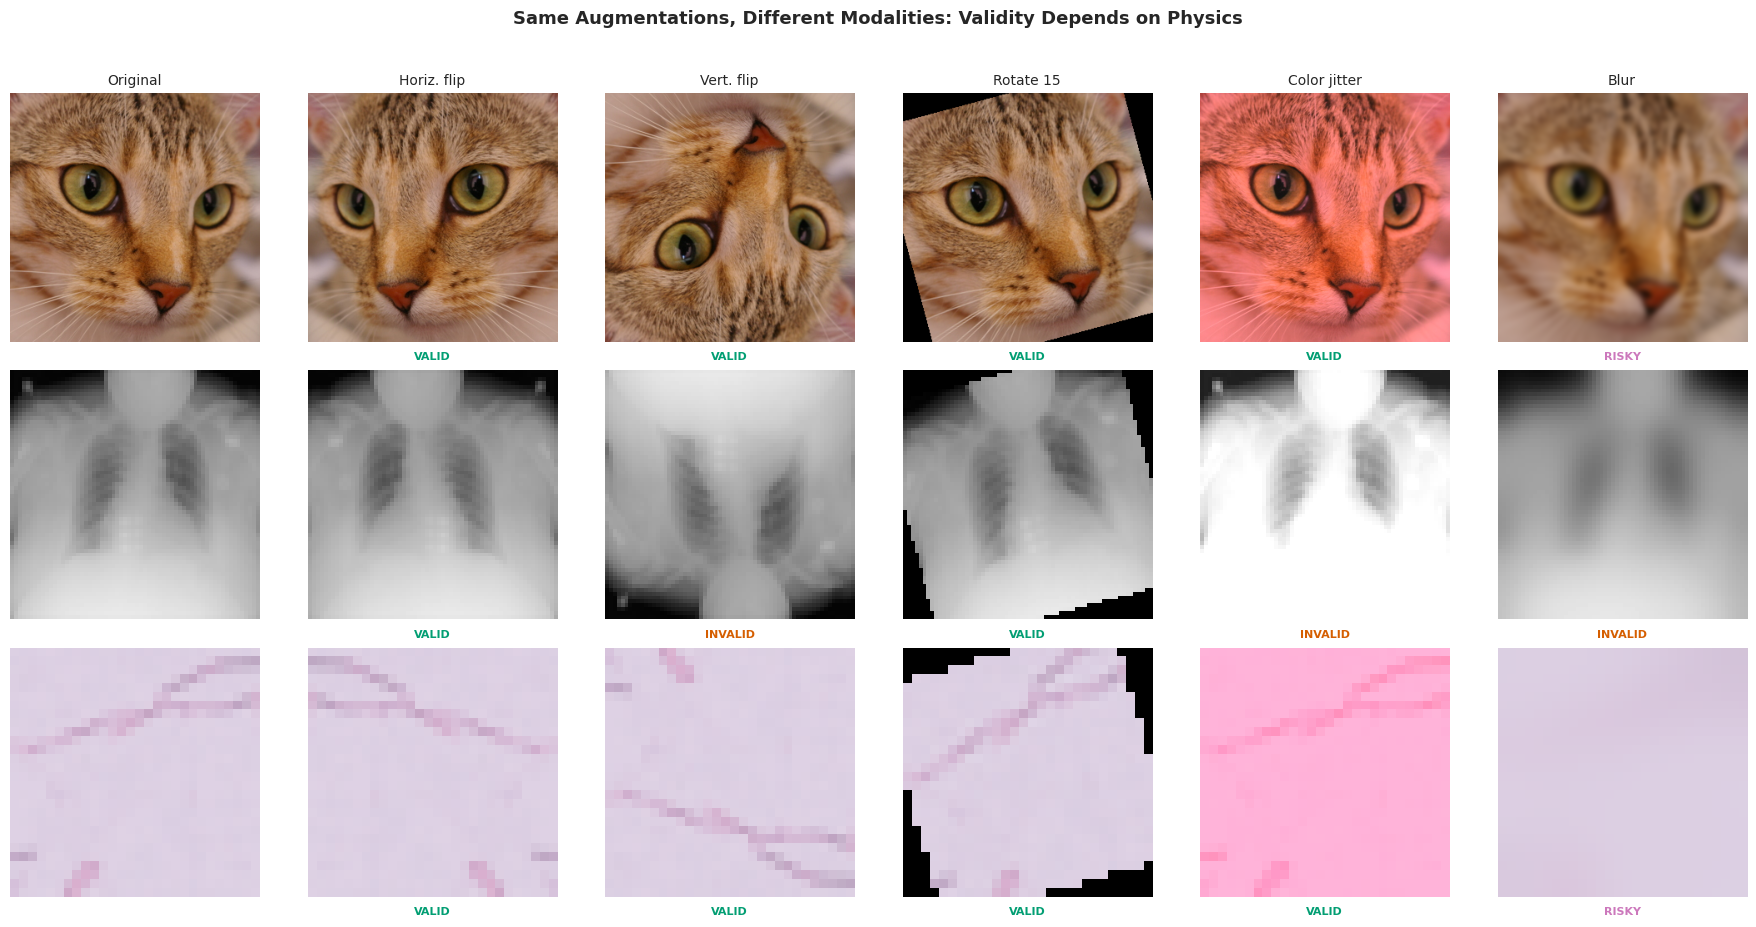
\includegraphics[width=\textwidth,height=0.66\textheight,keepaspectratio]{fig7_augmentation_comparison.png}
\end{center}
\vspace{-0.3em}
{\scriptsize Real images: natural (cat), chest X-ray (ChestMNIST), H\&E pathology (PathMNIST). Vertical flip: valid for pathology, invalid for X-ray. Color jitter: valid for pathology (stain variation), invalid for X-ray (intensity is the signal).}
\end{frame}

% ============================================================
\begin{frame}{Augmentation: Modality-Specific Reference}
\begin{center}
\renewcommand{\arraystretch}{1.3}
\begin{tabular}{lccc}
\toprule
\textbf{Augmentation} & \textbf{Chest X-ray} & \textbf{Pathology} & \textbf{Retinal Fundus} \\
\midrule
Horizontal flip & \textcolor{hlgreen}{\checkmark} (usually; laterality can matter) & \textcolor{hlgreen}{\checkmark} & \textcolor{columbiaaccent}{$\times$} (OD/OS) \\
Vertical flip & \textcolor{columbiaaccent}{$\times$} (up/down matters) & \textcolor{hlgreen}{\checkmark} & \textcolor{columbiaaccent}{$\times$} \\
Rotation $\pm 15^\circ$ & \textcolor{hlgreen}{\checkmark} & \textcolor{hlgreen}{\checkmark} & \textcolor{hlgreen}{\checkmark} \\
Color jitter & \textcolor{columbiagray}{$\sim$} (mild OK; intensity is signal) & \textcolor{hlgreen}{\checkmark} (stain var.) & \textcolor{hlgreen}{\checkmark} (camera) \\
Random crop & \textcolor{columbiagray}{$\sim$} (may lose finding) & \textcolor{hlgreen}{\checkmark} (tiles) & \textcolor{columbiagray}{$\sim$} \\
Gaussian blur & \textcolor{columbiaaccent}{$\times$} (hides fine detail) & \textcolor{columbiagray}{$\sim$} & \textcolor{columbiaaccent}{$\times$} \\
\bottomrule
\end{tabular}
\end{center}

\begin{block}{Lesson}
Blindly applying a natural-image augmentation pipeline can \emph{hurt} performance. Validate augmentations against clinical meaning. {\small (Notebook Fig.~6)}
\end{block}
\end{frame}

% ============================================================
\begin{frame}{Augmentation Ablation on Real X-Rays (Notebook Fig.~6)}
\centering
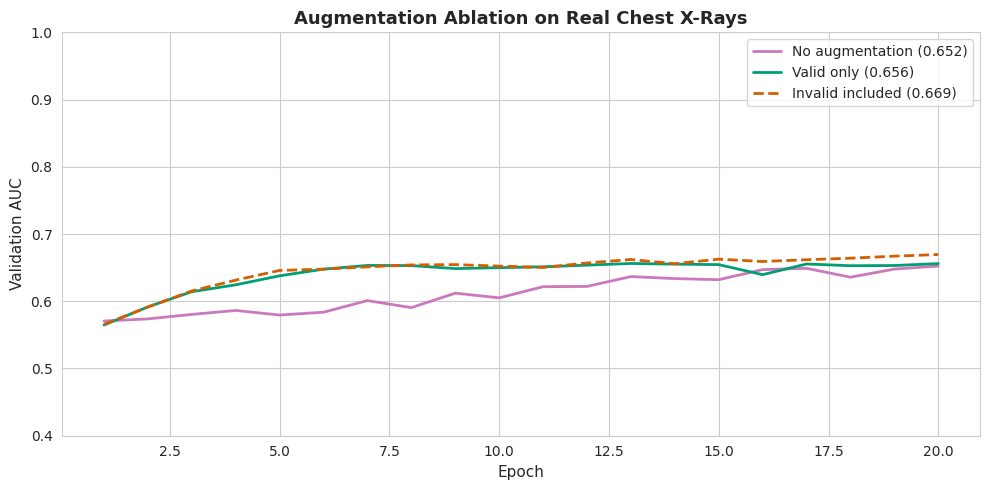
\includegraphics[width=0.80\textwidth]{fig6_augmentation_ablation.png}

\vspace{-0.3em}
{\scriptsize No augmentation vs.\ valid-only (horiz.\ flip + rotation) vs.\ invalid included (adds vert.\ flip + intensity jitter). Even ``invalid'' augmentations can help via data volume---but risk encoding false invariances.}
\end{frame}

% ============================================================
\section{Deployment Pitfalls}
% ============================================================
\begin{frame}{Multi-Site Generalization}
\textbf{Recall L21 (metadata):} Scanner manufacturer, field strength, and protocol differ across sites.

\begin{center}
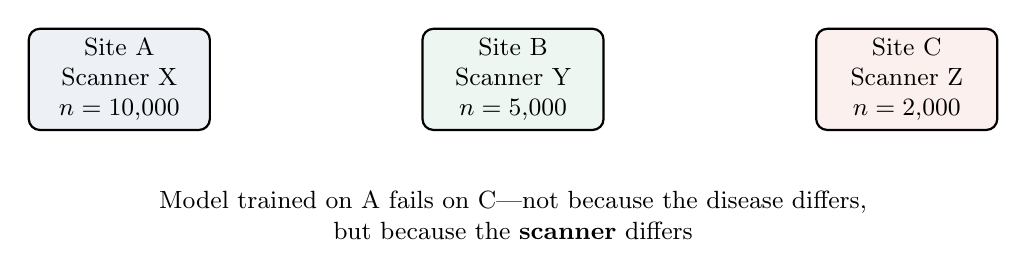
\begin{tikzpicture}[
    site/.style={draw,thick,rounded corners,minimum width=2.3cm,minimum height=1.1cm,align=center,font=\small},
    >=Stealth
]
\node[site,fill=columbia!8] (s1) at (0,0) {Site A\\Scanner X\\$n=10{,}000$};
\node[site,fill=hlgreen!8] (s2) at (5,0) {Site B\\Scanner Y\\$n=5{,}000$};
\node[site,fill=columbiaaccent!8] (s3) at (10,0) {Site C\\Scanner Z\\$n=2{,}000$};

\node[below=0.8cm,font=\small,align=center] at (5,-0.5) {Model trained on A fails on C---not because the disease differs,\\but because the \textbf{scanner} differs};
\end{tikzpicture}
\end{center}

\textbf{Mitigation:} Multi-site training, domain adaptation, external evaluation, per-site reporting.
\end{frame}

% ============================================================
\begin{frame}{The Garden of Forking Paths}
\textbf{Researcher degrees of freedom in medical imaging studies:}
\begin{enumerate}[<+->]
    \item Dataset split (random vs.\ patient-level vs.\ temporal)
    \item Preprocessing (resize, crop, normalize, \emph{window settings})
    \item Augmentation strategy
    \item Architecture and hyperparameters
    \item Evaluation metric and operating point
    \item Subgroup selection for reporting
\end{enumerate}

Each inflates performance by 1--5 AUC points. Compounded $\to$ ``superhuman AI'' hype.

\textbf{Recall L21 (pitfalls):} Shortcut learning (``PORTABLE'' text) is a \emph{predictable consequence} of the acquisition pipeline. The five-question framework helps anticipate these failures.
\end{frame}

% ============================================================
\section{Foundation Models}
% ============================================================

\begin{frame}{Foundation Models for Medical Imaging}
\textbf{The recent shift:} Large-scale pre-trained models are changing the field.

\begin{center}
{\footnotesize
\renewcommand{\arraystretch}{1.05}
\begin{tabular}{p{2.2cm}p{2.3cm}p{2.3cm}p{3.3cm}}
\toprule
\textbf{Model} & \textbf{Modality} & \textbf{Method} & \textbf{Key Idea} \\
\midrule
CheXzero & Chest X-ray & CLIP (img+text) & X-rays paired with reports \\
CONCH & Pathology & Contrastive & Tissue images + captions \\
BiomedCLIP & Multi-modal & CLIP & Broad biomedical img+text \\
SAM-Med & Multi-modal & Promptable seg. & Segment anything in med imgs \\
\bottomrule
\end{tabular}
}
\end{center}
\textbf{What this changes for the five-question framework:}
\begin{itemize}[<+->]
    \item \textbf{Transfer:} domain-specific pre-training at scale---addresses L21's physics gap
    \item \textbf{Labels:} zero-shot classification reduces labeling burden---but doesn't eliminate it
    \item \textbf{Pitfalls:} new failure modes (training data bias baked into the FM, harder to audit)
\end{itemize}

{\small FMs don't solve the label quality or evaluation problems---they change \emph{which} problems dominate.}
\end{frame}

% ============================================================
\section{Summary}
% ============================================================

\begin{frame}{Summary}
\begin{center}
\renewcommand{\arraystretch}{1.3}
{\small
\begin{tabular}{lp{3.3cm}p{2.8cm}p{3cm}}
\toprule
\textbf{Paradigm} & \textbf{Task} & \textbf{Architecture} & \textbf{Key Challenge} \\
\midrule
Classification & What does image show? & CNN + fine-tuning & Label noise, evaluation \\
Segmentation & Where exactly? & U-Net + variants & Boundary precision, 3D \\
MIL & Slide-level from tiles & Attention-MIL & Tile labels are \emph{wrong} \\
\bottomrule
\end{tabular}
}
\end{center}

\textbf{Decision rules for your next imaging project:}
\begin{itemize}[<+->]
    \item \textbf{First:} audit labels, check for shortcuts, plan external validation
    \item \textbf{Then:} choose architecture (U-Net for segmentation, MIL for WSI)
    \item \textbf{Augmentation:} reason from physics, not from ImageNet defaults
    \item \textbf{Transfer:} measure the benefit; don't assume it helps
\end{itemize}
\end{frame}

% ============================================================
\begin{frame}{Connections Backward}
\begin{itemize}[<+->]
    \item \textbf{L21 (Imaging Data):} Physics, economics, metadata, labels, pitfalls---predict every modeling challenge today
    \item \textbf{L17--18 (EHR):} Imaging as EHR events; Berkson's paradox explains shortcuts
    \item \textbf{L19--20 (NLP):} NLP on reports $\to$ silver-standard labels (the label quality problem)
    \item \textbf{ML Fundamentals:} CNNs, encoder-decoder, attention---today: where they break
    \item \textbf{Loss Functions:} CE from earlier; Dice loss new for segmentation
\end{itemize}
\end{frame}

% ============================================================
\begin{frame}{Companion Notebook}
\textbf{\texttt{nb22\_medical\_imaging\_modeling.ipynb}}:
\begin{enumerate}
    \item ImageNet features on natural image vs.\ chest X-ray (Fig.~1)
    \item Compare fine-tuning vs.\ lightweight models, Transfusion-inspired (Fig.~2)
    \item Train U-Net vs.\ no-skip baseline on real polyp data (Kvasir-SEG, Fig.~3)
    \item Compare loss functions: CE vs.\ Dice vs.\ combined (Fig.~4)
    \item MIL on real H\&E pathology tiles (PathMNIST, Fig.~5)
    \item Augmentation ablation: valid vs.\ invalid transforms (Fig.~6)
    \item Augmentation comparison: real medical vs.\ natural images (Fig.~7)
\end{enumerate}

\textbf{How to use:} Run all cells, then experiment. All outputs save to \texttt{figures/}.
\end{frame}

% ============================================================
\begin{frame}[standout]
    Questions?
\end{frame}

\end{document}
